\documentclass[11pt,a4paper]{article}
\usepackage[margin=2.3cm]{geometry}
\usepackage{amsmath,amssymb}
\usepackage{graphicx}
\usepackage{booktabs}
\usepackage{xcolor}
\usepackage{float}
\usepackage{caption}
\usepackage{enumitem}
\usepackage[colorlinks=true,linkcolor=blue!50!black,urlcolor=blue!50!black]{hyperref}
\graphicspath{{../results/figures/}}
\setlength{\emergencystretch}{3em}
\setlist{itemsep=3pt,topsep=4pt}

\newcommand{\cbox}[3]{\par\medskip\noindent\fcolorbox{#1!60!black}{#1!6}{%
  \begin{minipage}{\dimexpr\linewidth-2\fboxsep-2\fboxrule\relax}\textbf{#2}\enspace #3\end{minipage}}\par\medskip}
\newcommand{\keyidea}[1]{\cbox{blue}{Key idea.}{#1}}
\newcommand{\analogy}[1]{\cbox{teal}{Analogy.}{#1}}
\newcommand{\howtoread}[1]{\cbox{orange}{How to read this figure.}{#1}}
\newcommand{\takeaway}[1]{\cbox{violet}{Take-away.}{#1}}

\title{\textbf{When genes help one sex and harm the other}\\[4pt]
\large Testing evolutionary maths with virtual populations: a learner's guide}
\author{Companion to the expert report}
\date{5 October 2026}

\begin{document}
\maketitle

\begin{center}\begin{minipage}{0.88\linewidth}\small
\textbf{What this report is about.} Biologists use equations to predict how gene frequencies change over generations. We took the equations from a research poster and several classic papers. Separately, we built \emph{virtual populations of individual organisms} that are born, survive or die, mate and pass on genes, without ever being shown the equations. Then we checked whether those populations behave the way the equations predict. Mostly they do. Where they don't, the reason turned out to be interesting biology.
\end{minipage}\end{center}

\tableofcontents
\newpage

%=====================================================================
\section{The biology in one page}
\subsection{Sexual conflict inside a single gene}
Males and females often need different things: different body sizes, colours, behaviours or metabolisms. But they share almost the same genome. When one version of a gene (an \emph{allele}) is good for males and bad for females, or the reverse, the gene is \textbf{sexually antagonistic}. This tug-of-war within one gene is called \textbf{intra-locus sexual conflict (IaSC)}.

\analogy{Picture one thermostat shared by two roommates, one who likes it warm and one who likes it cold. Whatever setting wins, someone is unhappy. A gene with an antagonistic allele is a thermostat shared by the two sexes.}

\subsection{How could the conflict be resolved?}
One idea is a second gene, a \textbf{modifier}, that changes how strongly the first gene is \emph{expressed} in females. It could switch off the harmful allele in females only. Then the conflict would be ``resolved'': each sex gets roughly what it needs. Manas Samant and colleagues (IISER Mohali) built a mathematical model of exactly this, and that model is our main subject.

\subsection{Other papers in the folder}
\begin{itemize}
\item \textbf{Parsons (1961):} when can a brand-new allele spread, if its effects differ between the sexes?
\item \textbf{Owen (1953):} such a system can have \emph{two} different stable outcomes.
\item \textbf{Havird \emph{et al.}\ (2019):} mitochondria are inherited only from mothers, so a mitochondrial mutation that harms males but helps females can still spread. This is called ``mother's curse''.
\item \textbf{Morrow \emph{et al.}\ (2003):} experiments on how males harm females in insects. These are experiments rather than equations, so we used them only as background.
\end{itemize}

%=====================================================================
\section{Our approach: two independent engines}
\keyidea{If you only ever solve the equations, you can't tell whether the equations really describe a population of individuals. So we built two completely separate ``engines'' and compared their outputs.}

\begin{description}
\item[Engine 1, the oracle.] The paper's equations, computed exactly. Think of a perfectly large population with no randomness.
\item[Engine 2, the virtual population (IBM, ``individual-based model'').] Thousands of simulated organisms, each with genes and a sex. Every generation:
  \begin{enumerate}
  \item each individual survives with a probability set by its genes and sex;
  \item survivors pair up at random;
  \item babies inherit genes by Mendel's rules (or from the mother only, for mitochondria).
  \end{enumerate}
\end{description}

The crucial rule is \textbf{zero leakage}: the virtual population never sees the equations, not even the equilibrium they predict. The only things both engines share are the \emph{conditions} (how fit each genotype is, how often genes recombine, how big the population is). An automatic test checks that the simulation code never imports the maths.

\analogy{It is like testing a weather formula by building a miniature atmosphere out of individual air molecules. If the molecules swirl the way the formula says, the formula captures something real.}

\textbf{Why expect differences?} Real populations are finite, so chance matters. This randomness is called \textbf{genetic drift}. A coin tossed 10 times rarely gives exactly 5 heads; a population of 500 rarely keeps exactly the predicted gene frequency. The equations ignore drift, but the virtual population has it built in.

%=====================================================================
\section{The main model: can a modifier resolve the conflict?}
\subsection{The set-up}
\begin{itemize}
\item One gene has two alleles. $A_1$ helps males (fitness $1+a$) and $A_2$ helps females (fitness $1+b$).
\item A second gene carries a modifier, $M_1$, that changes how the alleles act in females. $k_1$ is how much $M_1$ protects females from the harmful $A_1$; $k_2$ is how much of $A_2$'s female benefit survives.
\item $r$ is how often the two genes get shuffled apart at reproduction (recombination).
\end{itemize}

\subsection{What we found in the maths}
\begin{enumerate}
\item The conflict keeps both alleles in the population at a balance point $p^*=\tfrac12+\tfrac12(1/b-1/a)$, exactly the formula on the poster. This only works when the male and female benefits are similar in size (for $b=0.2$, $a$ must lie between $1/6$ and $1/4$).
\item Whether a new modifier can invade depends on $k_1$, $k_2$, $a$, $b$ and $r$. We rebuilt every heatmap and diagram on the poster. The points where the modifier starts to win match the poster to within about 0.002.
\item We found a simple explanation for the poster's observation that \textbf{low recombination helps resolution}:
  \begin{itemize}
  \item when the modifier stays attached to the $A_1$ allele (no shuffling), it is always helping the females it protects, so it always spreads;
  \item shuffling moves it onto $A_2$, where it only gets in the way.
  \end{itemize}
\end{enumerate}

\begin{figure}[H]\centering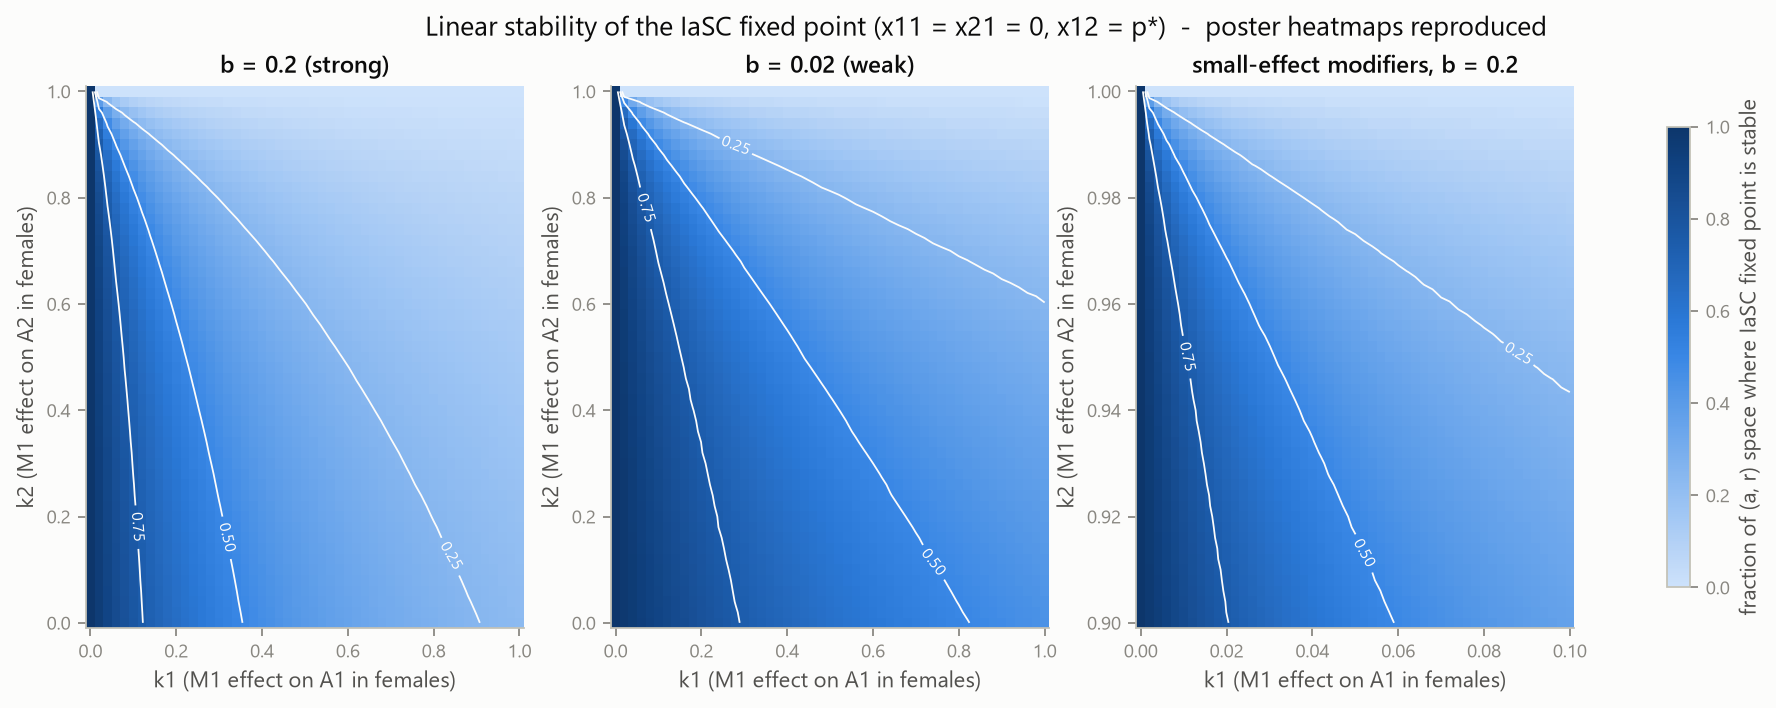
\includegraphics[width=\textwidth]{P1_stability_heatmaps.png}
\caption{Where does the conflict persist?}\end{figure}
\howtoread{Each square is one kind of modifier ($k_1$ across, $k_2$ up). Dark means the conflict usually persists (the modifier fails); light means the modifier usually wins. Modifiers that protect females strongly ($k_1$ large) succeed most. Weaker selection (middle panel) makes resolution harder.}

\subsection{What the virtual populations did}
\begin{itemize}
\item They settled at the predicted balance point. Large populations (5{,}000) were within about 2\% on average; small ones (500) wandered much more.
\item When we added the modifier, it spread exactly where the equations said it should, in \textbf{99\%} of the cases with a clear outcome.
\item Two things the equations cannot show:
\end{itemize}
\begin{enumerate}
\item \textbf{The conflict itself can vanish by chance.} The force holding the two alleles in balance is extremely weak (a ``restoring'' factor of 0.992 to 0.99997, where 1 means no force at all). In small populations drift often removes one allele before any modifier can act.
\item \textbf{Sharp thresholds become probabilities.} Sometimes the maths says ``the modifier wins only if it starts above 41\%''. Virtual populations instead show a smooth S-shaped curve of success, and the curve gets sharper in bigger populations.
\end{enumerate}

\begin{figure}[H]\centering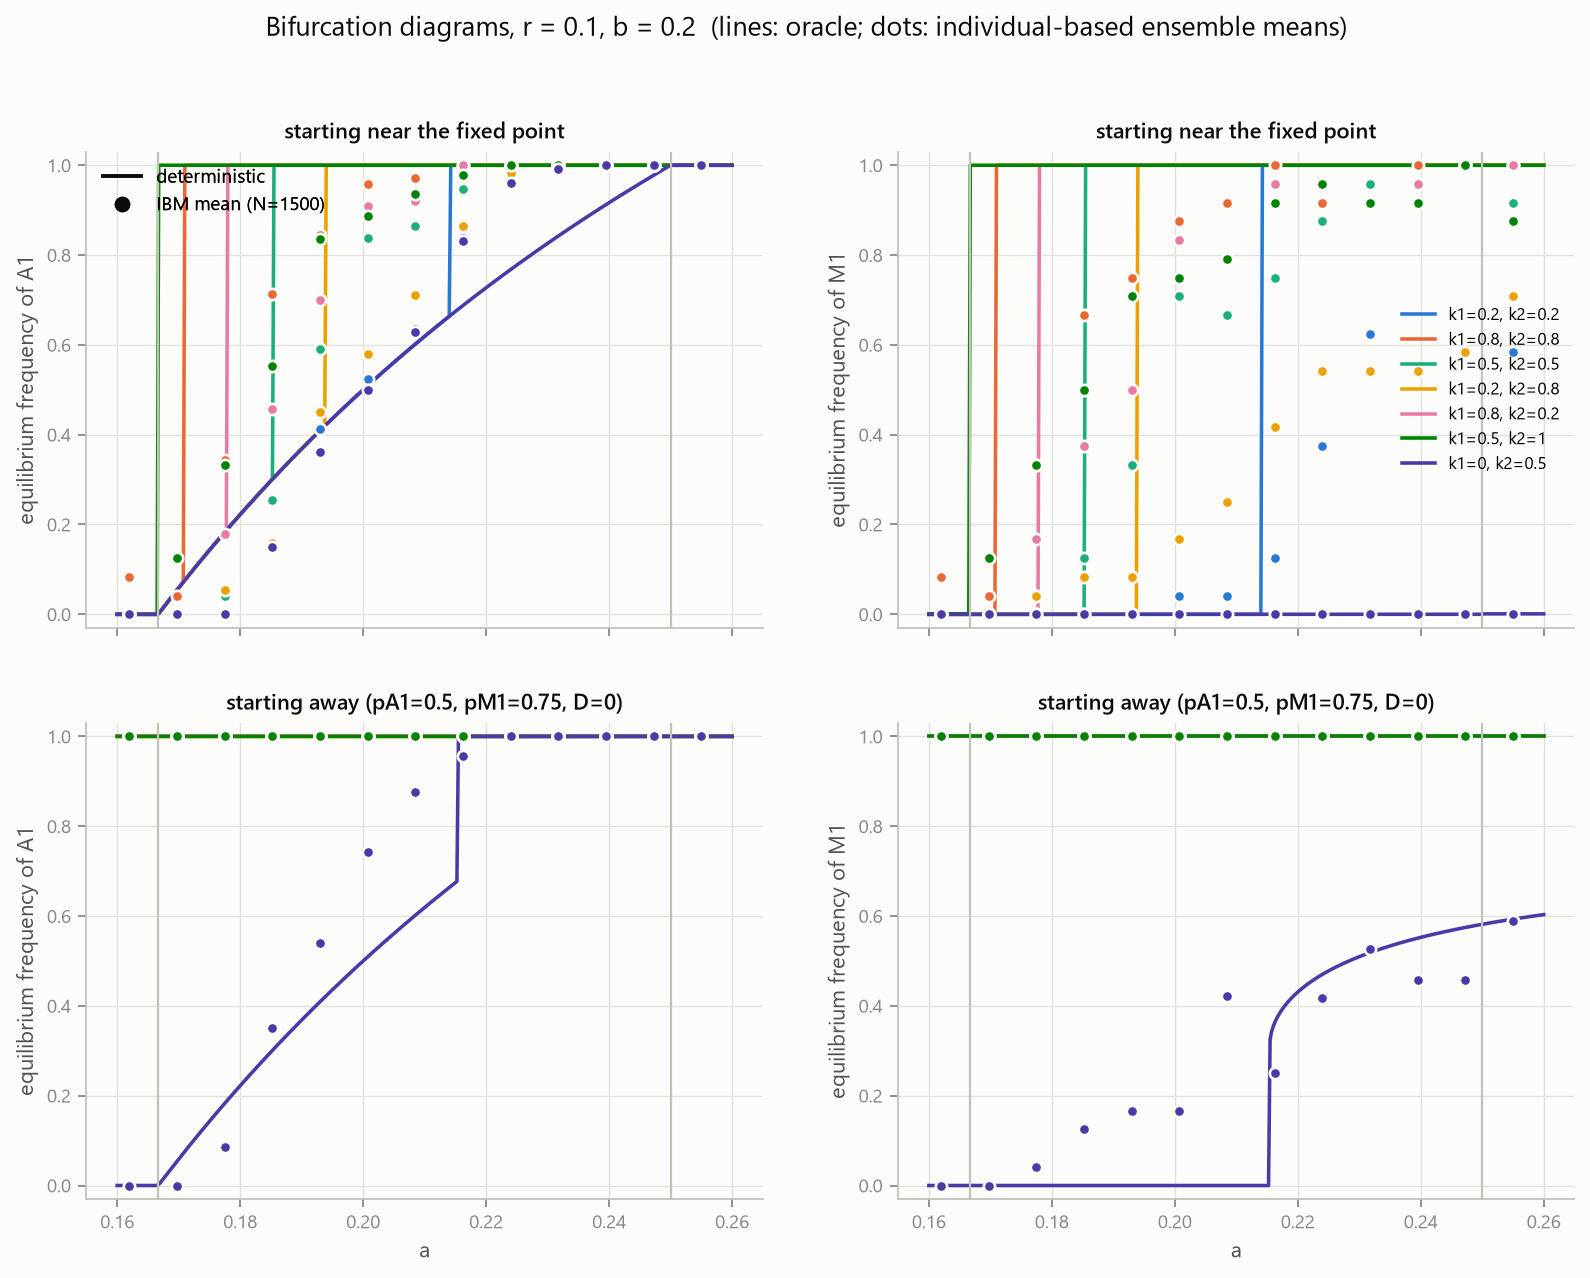
\includegraphics[width=0.85\textwidth]{P3_bifurcation.png}
\caption{Final gene frequencies as the male benefit $a$ increases.}\end{figure}
\howtoread{Lines are the equations; dots are averages over many virtual populations. Each colour is one type of modifier. Where a line jumps from 0 to 1, the maths says ``the modifier now always wins''. The dots rise more gradually, because in a finite population a winning modifier can still be lost by bad luck while it is rare.}

\begin{figure}[H]\centering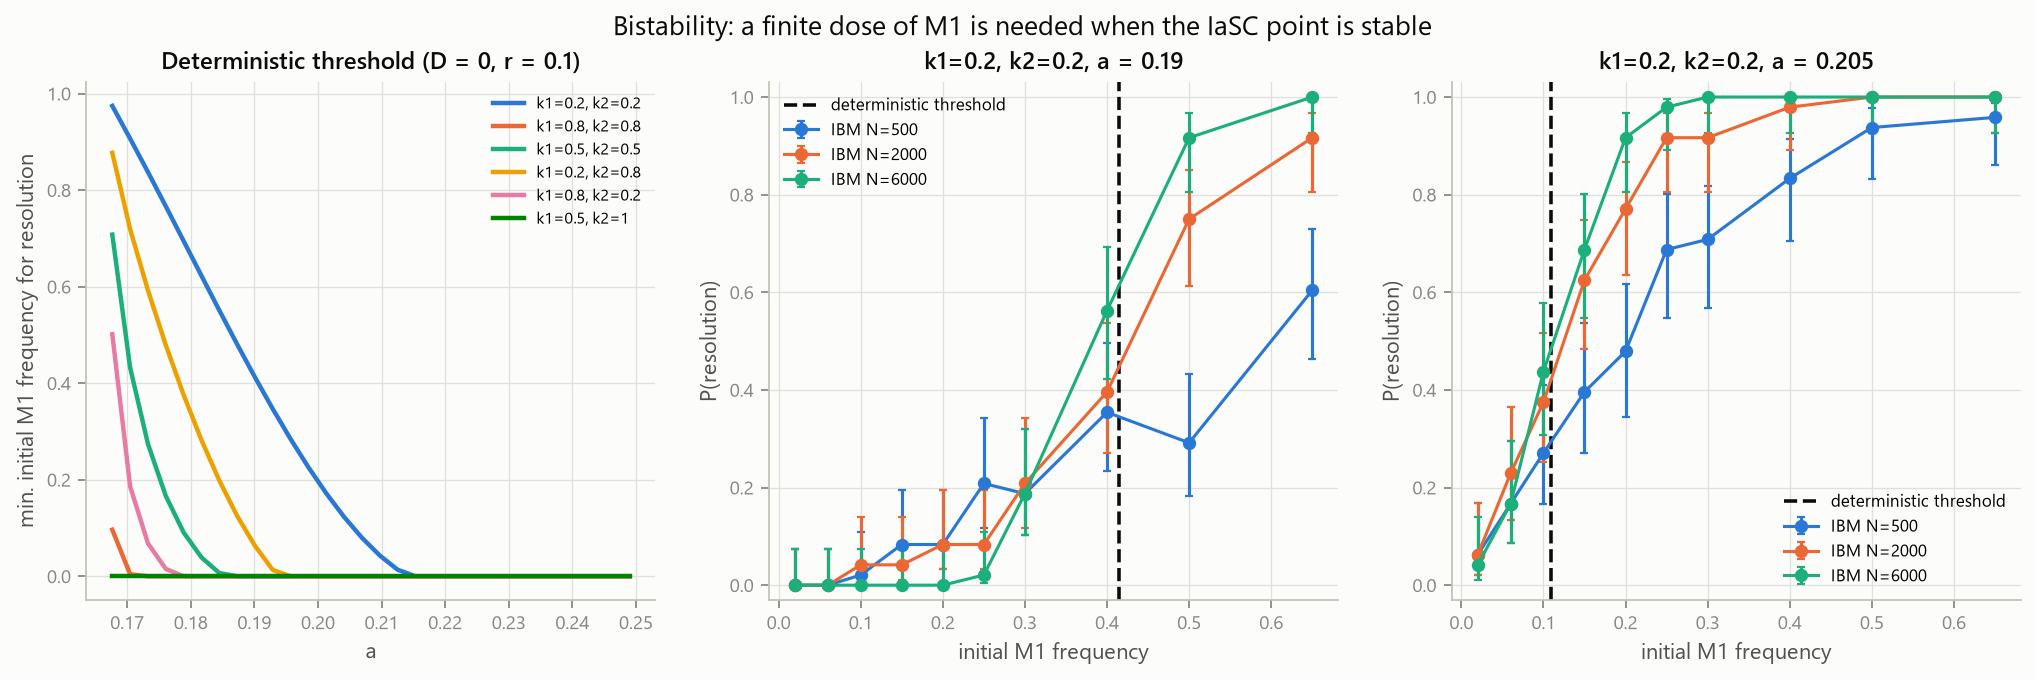
\includegraphics[width=\textwidth]{P4_thresholds.png}
\caption{How much modifier is needed?}\end{figure}
\howtoread{Middle and right: the dashed line is the minimum starting amount the maths requires. Coloured curves show how often virtual populations succeed. Bigger populations (green) get closer to a sharp step at the dashed line.}

\takeaway{The poster's conclusions hold up. Our virtual populations add a caveat: in small populations the conflict may disappear by chance before a modifier can resolve it.}

%=====================================================================
\section{Parsons and Owen: can a new allele get started?}
\begin{itemize}
\item Parsons showed a simple rule: a new allele spreads if its average advantage across the two sexes, in carriers that have one copy, is positive. More precisely, the two sexes' ``heterozygote advantages'' must add up to more than 2. So an allele can spread even if it hurts one sex, as long as it helps the other sex more.
\item For genes on the X chromosome (males have only one copy), the rule changes.
\item Owen showed that some fitness combinations give \emph{two} possible stable endpoints, like a ball that can rest in either of two valleys.
\end{itemize}

\textbf{Results.}
\begin{itemize}
\item The virtual populations obeyed Parsons' rule in \textbf{100\%} of clear cases, for both normal and X chromosomes.
\item Parsons' worked example: the equations predict a final frequency of 0.4399; the virtual populations gave 0.4402.
\item In Owen's two-valley system, every starting point ended in the valley the maths predicts.
\end{itemize}

\begin{figure}[H]\centering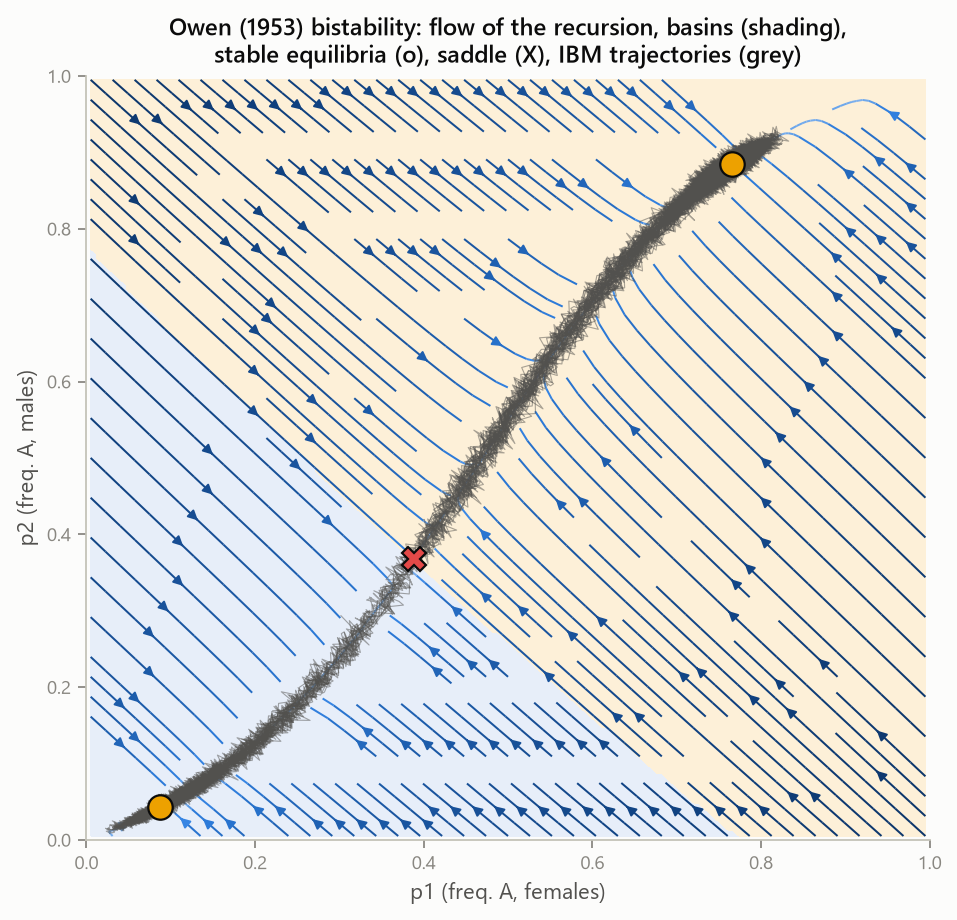
\includegraphics[width=0.55\textwidth]{O4_owen_phase_portrait.png}
\caption{Owen's two valleys.}\end{figure}
\howtoread{The axes are the allele's frequency in females and in males. Blue streamlines show where the equations push a population. The two orange dots are the valleys (stable endpoints) and the red X is the ridge between them. Grey squiggles are real virtual populations wandering towards one valley or the other.}

%=====================================================================
\section{Mother's curse}
\begin{itemize}
\item Mitochondria are passed on only by mothers, so natural selection cannot ``see'' what a mitochondrial mutation does to males.
\item \textbf{Prediction 1.} A mutation that helps females even slightly will spread however much it harms males. The virtual populations confirmed this: how fast the mutation spread was statistically the same whether males paid nothing or lost 90\% of their fitness.
\item \textbf{Prediction 2, the ``twofold rule''.} If the same male-sterilising mutation were in the nucleus (inherited from both parents), it would need to \emph{double} female fitness to spread. We showed that this follows directly from Parsons' 1961 rule, and the virtual populations agreed in 94\% of cases.
\item \textbf{Prediction 3, the arms race.} Nuclear ``restorer'' genes that protect males should then spread. They did in 94--100\% of populations, but only when the harmful mitochondria were present.
\end{itemize}

\begin{figure}[H]\centering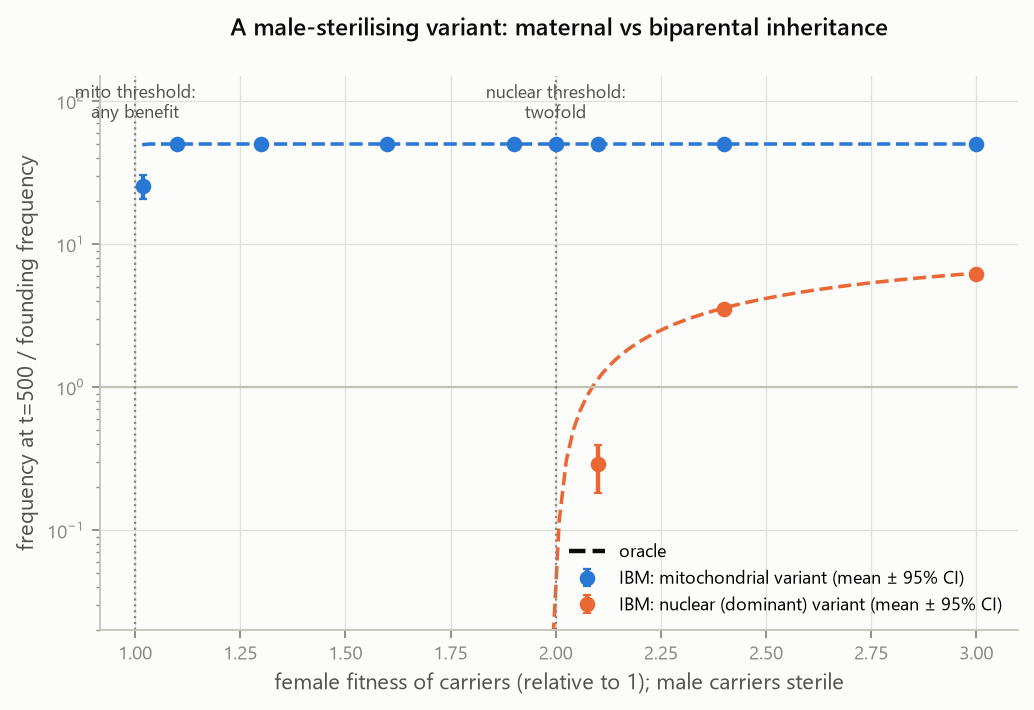
\includegraphics[width=0.6\textwidth]{C2_twofold_rule.png}
\caption{The twofold rule.}\end{figure}
\howtoread{Blue: a mitochondrial variant spreads with any female benefit. Orange: the nuclear version only starts spreading once female fitness passes 2 (twice normal).}

%=====================================================================
\section{More tests from the wider literature}
\subsection{Where in the genome can conflict survive? (Kidwell, Rice, Fry)}
\begin{itemize}
\item In 1984, Rice argued that the X chromosome should be a hotspot for antagonistic genes.
\item In 2010, Fry showed that this depends on \emph{dominance}: whether one copy of an allele has a full effect or only a partial one.
\item We tested three dominance scenarios on normal chromosomes and on the X. The virtual populations agreed with the published conditions in \textbf{98--100\%} of cases, and reproduced the whole debate:
  \begin{itemize}
  \item the X wins only when the male-helping allele is recessive;
  \item normal chromosomes win otherwise.
  \end{itemize}
\end{itemize}

\begin{figure}[H]\centering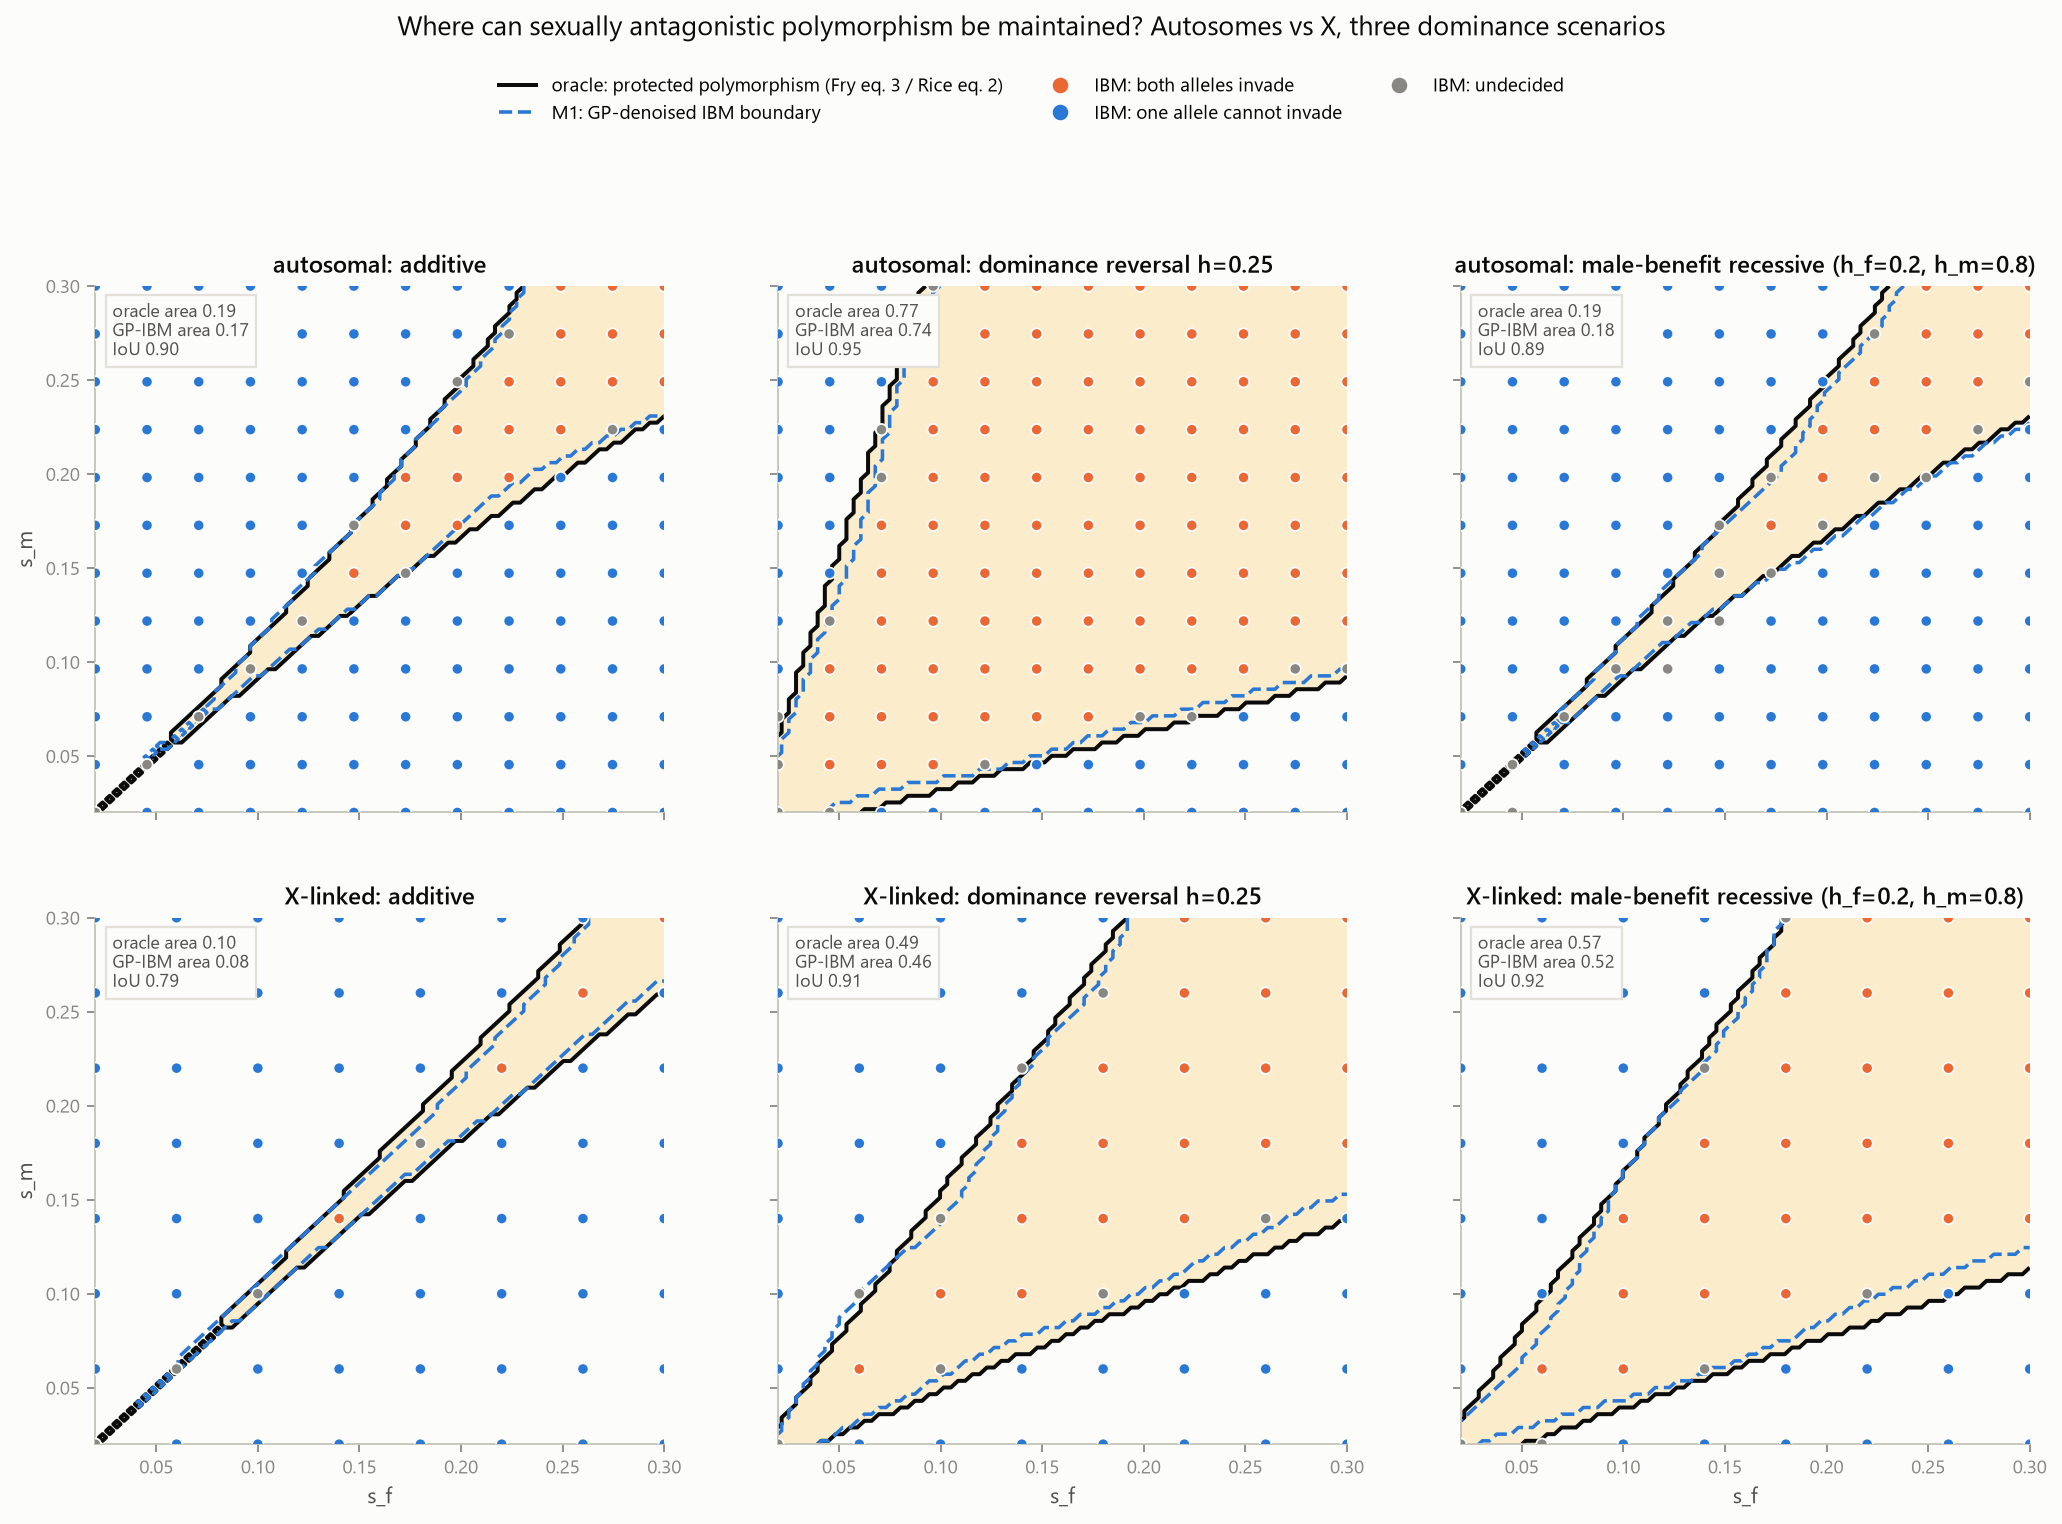
\includegraphics[width=\textwidth]{E1_E2_polymorphism_maps.png}
\caption{Where both alleles can coexist.}\end{figure}
\howtoread{Axes are how strongly selection acts in females ($s_f$) and males ($s_m$). The shaded wedge is where theory says both alleles survive. Orange dots: virtual populations kept both. Blue dots: one allele was lost. The dashed blue line is the boundary that a machine-learning smoother extracted from the virtual-population results alone. It hugs the theory line, staying slightly inside because chance trims the edges.}

\subsection{Chance of an allele taking over (Kimura)}
Kimura's famous 1962 formula gives the probability that an allele eventually takes over a finite population.
\begin{itemize}
\item It matched the virtual populations very well when both sexes favour the allele, and for mitochondrial variants. For mitochondria the effective population is only the mothers, so chance is twice as strong.
\item When the two sexes pull \emph{strongly} in opposite directions, the usual shortcut (``just average the two sexes'') failed. A more complete version of the same theory fixed it. This is a nice example of the virtual population revealing the limits of a textbook formula.
\end{itemize}

\subsection{Genes near the sex-determining region (Rice 1987)}
If an antagonistic gene sits right next to the gene that makes an individual male, the male-helping allele can ride on the Y chromosome and the female-helping one on the X. Then both survive. We built virtual populations in which sex is genuinely inherited through the Y. They matched the theory in \textbf{96\%} of cases, including how strongly the Y and X differ.

\subsection{How long does the conflict last?}
Using diffusion theory, a mathematical description of drift, we predicted how many generations the poster's conflict survives in a finite population. After measuring the virtual population's \emph{effective} size (about 90\% of its actual size, because random deaths add extra noise), the predictions came within about 4\% of the simulated times. In mid-range conditions the survival time grows very fast with population size: about 500 generations at 200 individuals but about 38{,}000 at 800.

%=====================================================================
\section{Where machine learning came in}
We used ML only to \emph{analyse} results, never inside the virtual population.
\begin{description}
\item[Denoiser.] Simulation results are noisy. A Gaussian-process model smoothed them and drew the boundary of the ``coexistence'' region. It overlapped the textbook region by 79--96\%, better than the raw results.
\item[Emulator.] A small neural network learned fixation probabilities from simulations of small populations, then predicted a larger population it had never seen. It succeeded only when given the ``right'' combination of inputs (population size times selection strength), which is exactly the combination Kimura's theory says matters. In effect the data rediscovered the theory.
\item[Detective.] From one simulated history of gene frequencies, we tried to work out how strong selection was in each sex. A network trained on simulations did this 2.5--3 times more accurately than fitting the original equations, because it had learned how drift distorts the data.
\end{description}

%=====================================================================
\section{Behind the scenes}
\begin{itemize}
\item Everything is written in Python, with fast compiled code (numba). There is an optional mode that runs the virtual populations on the AMD graphics card, about 7--10 times faster.
\item Simulations ran at low priority, leaving room for other work on the same laptop.
\item 36 automatic tests check correctness, including that the simulation never peeks at the equations.
\item All numbers, tables and figures can be regenerated with one command.
\end{itemize}

%=====================================================================
\section{The big picture}
\begin{enumerate}
\item The equations in the poster and the classic papers really do describe what happens in populations of individuals, as long as their assumptions hold.
\item The differences we found all come from \textbf{chance in finite populations}, and a more complete stochastic theory predicts each of them.
\item For the poster's question: modifiers can resolve sexual conflict much as the model says. In small populations, though, the conflict may disappear by drift before a modifier gets the chance.
\end{enumerate}

\subsection*{Questions still open for the poster's authors}
\begin{itemize}
\item Exactly what life cycle (order of selection, mating and recombination) was assumed?
\item What range of parameters does ``fraction of parameter space'' mean?
\item What starting point was used for the ``away from the fixed point'' plot?
\end{itemize}

%=====================================================================
\section*{Glossary}
\begin{description}[itemsep=2pt]
\item[Allele] One version of a gene.
\item[Antagonistic (sexually)] Good for one sex, bad for the other.
\item[Bistability] Two possible stable outcomes; which one you reach depends on where you start.
\item[Diffusion theory] Maths that describes gene frequencies wandering randomly under drift and selection.
\item[Dominance] How much one copy of an allele does compared with two copies.
\item[Drift] Random change in gene frequencies because populations are finite.
\item[Effective population size ($N_e$)] The size of an idealised population that has the same amount of drift.
\item[Equilibrium] A gene frequency at which nothing changes any more.
\item[Fixation] An allele reaching 100\% frequency.
\item[Heterozygote] An individual carrying two different alleles of a gene.
\item[IBM] Individual-based model: a simulation of individual organisms.
\item[Invasion] A rare new allele increasing in frequency.
\item[Modifier] A gene that changes how another gene is expressed.
\item[Oracle] Our name for the exact solution of the paper's equations.
\item[Polymorphism] Two or more alleles coexisting in a population.
\item[Recombination ($r$)] Shuffling of genes between chromosomes during reproduction.
\item[Zero leakage] Our rule that the simulation never uses the paper's equations.
\end{description}
\end{document}
